% Original vector reconstruction: source Fig.49.2, PDF211 / printed199.
% S49-G02-t, S49-G02-u, S49-G02-s: relative coefficients +,-,+.
% All scalar internal lines remain vertical; arrows specify their momenta.
% Majorana arrows specify continuous matrix-chain orientations, not particle flow.
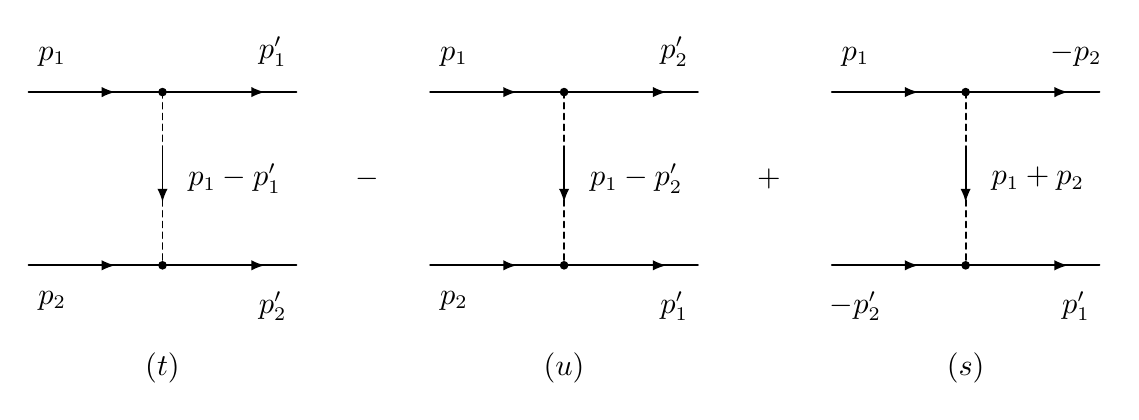
\begin{tikzpicture}[x=1mm,y=1mm,line width=.7pt,>=latex,
  line cap=round,line join=round,font=\fontsize{10.5}{12}\selectfont,
  scalar/.style={dash pattern=on 2.1pt off 1.8pt}]
  % t channel: p1 -> p1prime above; p2 -> p2prime below.
  \foreach \shift/\righttop/\leftbottom/\rightbottom/\momentum/\channel in {
    0/{p'_1}/{p_2}/{p'_2}/{p_1-p'_1}/t,
    51/{p'_2}/{p_2}/{p'_1}/{p_1-p'_2}/u,
    102/{-p_2}/{-p'_2}/{p'_1}/{p_1+p_2}/s}{
    \begin{scope}[shift={(\shift,0)}]
      \foreach \y in {0,-22}{
        \draw (0,\y)--(34,\y);
        \draw[->] (4,\y)--(11,\y);
        \draw[->] (23,\y)--(30,\y);
        \fill (17,\y) circle[radius=.55mm];
      }
      \draw[scalar] (17,0)--(17,-22);
      \draw[->] (17,-7)--(17,-14);
      \node[above] at (3,2) {$p_1$};
      \node[above] at (31,2) {$\righttop$};
      \node[below] at (3,-24) {$\leftbottom$};
      \node[below] at (31,-24) {$\rightbottom$};
      \node[right] at (19,-11) {$\momentum$};
      \node at (17,-35) {$(\channel)$};
    \end{scope}
  }
  \node at (43,-11) {$-$};
  \node at (94,-11) {$+$};
\end{tikzpicture}
